\documentclass{report}
\usepackage{lipsum}
\usepackage{gensymb}
\usepackage{float}
\usepackage{graphicx} % Required for inserting images

\usepackage{cite}

\usepackage{graphicx}
\usepackage{svg}
\usepackage{xcolor}
\usepackage{tikz}
\usepackage{hyperref}
\usepackage{multirow}
\usepackage{enumerate}
\usepackage[shortlabels]{enumitem}
\usepackage{amsmath}
\usepackage{nomencl} % For nomenclature and acronyms
\makenomenclature % Activate nomenclature

\definecolor{lightblue}{HTML}{a0d8ef}

\title{Cryptanalysis - Biclique Attack Report} %title of the file

\begin{document}

%----------- Report information ---------

\logo{logos/ULB_round.png}
\uni{\textbf{Université Libre de Bruxelles}}
\ttitle{Biclique Attack on AES-128} %title of the file
\subject{INFO-F-537: Cryptanalysis} % Subject name
\topic{Project Report} % Topic name

\professor{Prof. \textsc{Van Assche} Gilles} % information related to the professor

\students{\textsc{Amanor} Deborah\\
          \textsc{Hassani} Mortaza} % information related to the students

%----------- Init -------------------

\buildmargins % display margins
\buildcover % create the front cover of the document
\toc % creates the table of contents

%------------ Report body ----------------

\section{Introduction}
The \textbf{biclique attack} is an advanced variant of the \textbf{Meet-in-the-Middle} (MITM)\nomenclature{MITM}{Meet-in-the-Middle} attack, for the cryptanalysis of block ciphers to recover secret keys. It addresses the limitations of the traditional MITM attack, which is limited in breaking ciphers without independent key bits. In a biclique attack, the process begins by partitioning all possible secret keys into groups. For each group, a biclique structure is constructed. This structure helps in filtering out incorrect keys through partial matching, leaving candidate keys. A valid \emph{plaintext-ciphertext pair (P, C)} is used to determine the correct key. Since biclique cryptanalysis is based on MITM attacks, it is applicable to most block ciphers. In this report, we will focus on the biclique attack applied to the full AES block cipher. 

\nomenclature{AES}{Advanced Encryption System}AES has been one of the most widely used and trusted block ciphers for decades. Despite several cryptanalysis efforts, no significant progress has been made in recovering the secret key of the full round AES with a computational complexity less than exhaustive key search. This is because AES was designed to withstand differential and linear cryptanalysis. \cite{bogdanov2011biclique} 

Impossible Differential Cryptanalysis was the first method to successfully attack a reduced version of AES, specifically targeting 7 rounds of AES-128. Similarly, the Square Attack was able to break 8 rounds of AES-192. These attacks, however, have not been able to extend to the full rounds of AES \cite{bogdanov2011biclique}. 

Currently, the only attack known to break the full rounds of AES faster than exhaustive key search is the biclique attack, introduced in 2011 by Bogdanov et al\cite{bogdanov2011biclique}. This attack represented a breakthrough in cryptanalysis of the AES block cipher by achieving key recovery of the full rounds with the following reduced computational complexities: 

\begin{table}[h!]
    \centering
    \begin{tabular}{|p{3cm}|p{3cm}|p{3cm}|}
        \hline
        \multicolumn{3}{|c|}{Computation Operations} \\
        \hline
        AES & Brute Force & Biclique \\
        \hline
        128 & $2^{128}$ & $2^{126.18}$ \\
        \hline
        192 & $2^{192}$ & $2^{189.74}$ \\
        \hline
        256 & $2^{256}$ & $2^{254.42}$ \\
        \hline
    \end{tabular}
    \caption{Biclique key recovery for AES\cite{bogdanov2011biclique}}
    \label{table:1}
\end{table}
% \begin{itemize}
%     \item     AES-128: 2\textsuperscript{126.18}  operations
%     \item     AES-192: 2\textsuperscript{189.74}  operations  
%     \item     AES-256 and 2\textsuperscript{254.42} operations
% \end{itemize}

While biclique cryptanalysis breaks the full AES, this is a theoretical attack and does not pose a practical threat due to its high computational complexity. In this report, we provide a detailed explanation of: 
\begin{enumerate}
    \item     The concept and construction of Bicliques 
    \item     The general Biclique Attack 
    \item     The application of the Biclique attack on AES block cipher 
    \item     An implementation of the attack on a reduced version of AES. 
\end{enumerate}

\newpage
\section{Background}
The concept of bicliques was first introduced in the cryptanalysis of hash functions. It originates from the \emph{splice-and-cut} framework in hash function cryptanalysis, more specifically its element called initial structure. The biclique approach led to the best preimage attacks on the SHA family of hash functions so far, including the attack on 50 rounds of SHA-512, and the first attack on a round-reduced Skein hash function. \cite{bogdanov2011biclique} 

 

The biclique attack is a variant of the \emph{meet-in-the-middle} (MITM) attack. 
It utilizes a biclique structure to extend the number of rounds that can be attacked compared to the basic MITM attack. 
In mathematics, a biclique is a special type of \textbf{bipartite graph} where every vertex of the first set is connected to every vertex of the second set. \cite{wikipedia_bipartite_graph}. 
It can be denoted as \(K_{mn}\), where $m$ is the number of vertices in the first set and $n$ is the number of vertices in the second set. 

\begin{figure}[h]
    \centering
    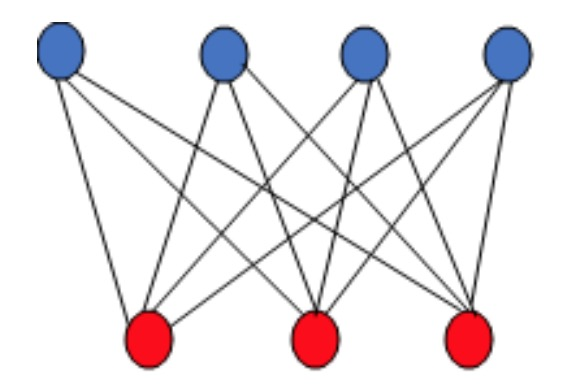
\includegraphics[width=0.25\textwidth]{figures/1.jpg}
    \caption{biclique with m=4 and n=3}
    \label{fig:biclique with m=4 and n=3}
\end{figure}
% \nomenclature{ABC}{Abbreviation Example}

Since the biclique attack builds on the principles of the MITM attack, we briefly describe the basic MITM attack to provide foundational context. 

\subsection{The Basic MITM}
The MITM attack is a time-memory trade of attack which is applied on block ciphers with independent key bits. This means that the keys used for encryption and decryption do not rely on each other, making block ciphers with multiple encryption rounds, such as double \nomenclature{DES}{Data Encryption Standard}DES (2DES), particularly vulnerable. For instance, in double DES, with a key size of $2^{112}$, MITM reduces the computational complexity of recovering the key from $2^{112}$ by using exhaustive key search to $2^{57}$ \cite{wikipedia_meet_in_the_middle}. 

However, due to the key scheduling and subkey dependencies of AES, where keys for different rounds are derived from each other, MITM is not effective. And as such, the number of AES rounds that can be broken using this technique is relatively small. 

For a block cipher with a key size $2^n$, an adversary partitions the key space into groups of size $2^{\text{d}} \times 2^{\text{d}}$, where \(n = 2d\). The keys are represented as a matrix \(K[i, j]\), and the cipher is divided into two sub-ciphers\cite{bogdanov2011biclique}: $g_1$ representing the forward computation and $g_2$ backward computation. 
\subsubsection{Steps in the MITM Attack\cite{bogdanov2011biclique}}
\begin{enumerate}
    \item \textbf{Forward Computation} The adversary encrypts the known plaintext $P$ using all possible values of the first key subset $2^d$. The intermediate values $V_{i}$ are computed and stored alongside the corresponding key values
    \\
    \begin{equation}
        g_1 = ENC_{k_1}(p)
    \end{equation}

    \begin{equation}
        P \xrightarrow[\quad g_1 \quad]{K[i, \cdot]} v_i
    \end{equation}

    \item 	\textbf{Backward Computation} The adversary decrypts the known ciphertext using all possible values of the second key subset $2^{d}$. The Intermediate values $V_j$ are computed and stored alongside their respective keys
        \begin{equation}
            g_2 = DEC_{k_2}(C)
        \end{equation}

        \begin{equation}
            v_j \xleftarrow[\quad g_2 \quad]{K[\cdot, j]} C
        \end{equation}


    \item	\textbf{Matching} The adversary compares the intermediate values, $V_{i}$  and $V_{j}$ to find a match. If \(V_i = V_j\) , then \(K[i, j]\) are the candidate key pairs

\end{enumerate}
The basic meet-in-the-middle attack has clear limitations in AES cipher cryptanalysis since an intermediate value can be found for a very small number of rounds only. Biclique cryptanalysis overcomes these limitations by introducing a more advanced structure, enabling attacks on the full AES.

\section{The Biclique Attack}
A \textbf{biclique} is a mathematical structure used in cryptanalysis of block ciphers to efficiently explore relationships between keys, plaintexts, and ciphertexts in a cipher. It connects $2^d$ intermediate states $\{S_j\}$ to $2^d$ Ciphertexts $\{C_i\}$ using $2^{2d}$ keys represented as $K[i, j]$. Each key $K[i, j]$ maps an intermediate state $\{S_j\}$ to a ciphertext $\{C_i\}$ through a subcipher $f$, mathematically expressed as\cite{bogdanov2011biclique}:
\begin{equation}
    \forall i, j : S_j \xrightarrow[\quad f \quad]{K[i, j]} C_i
    \label{eq:stateToCipher}
\end{equation}


\begin{equation}
C_i = f_{K[i, j]}(S_j), \forall i, j \in \{0, \ldots, 2^d - 1\}
\end{equation}
A biclique is then said to be d-dimensional if it connects $2^d$ intermediate states to $2^d$ ciphertexts. The dimension d determines the size and complexity of the structure. 

\subsection{Preliminary Steps}
To conduct the attack, the adversary performs two preparatory steps; Key partitioning and Cipher splitting.

\begin{enumerate}
    \item \textbf{Key Partitioning:}
    The adversary firstly partitions the key space of the cipher into subsets or groups of size $2^{2d}$ for some $d$, where the keys are represented as $K[i, j]$ in a matrix $2^d \times 2^d$ similar to that of the MITM\cite{bogdanov2011biclique}.

    \item \textbf{Cipher splitting}
    The adversary then splits the cipher into two subciphers, $f$ and $g$ such that the encryption process $e$ can be expressed as:
    
    \begin{equation}
        e = f \circ g
    \end{equation}
    
\end{enumerate}
Where $g$ maps the plaintext $P$ to an intermediate state $S$, and $f$ maps the intermediate state $S$ to the ciphertext $C$\cite{bogdanov2011biclique}.


\subsection{Constructing bicliques}
\label{sec:constructing_bicliques}
After completing the preliminary steps, the next phase involves constructing the biclique. Bogdanov et al. proposed two primary methods for biclique construction: Independent Related-Key Differentials and Interleaving Related-Key Differentials.

However, for the purpose of this study, we will focus only on the Independent Related-Key Differentials approach.

\subsubsection{Naïve Approach or Bruteforce}
A straightforward way to construct the biclique is to use the naive approach or brute-force method. This can be achieved when the adversary maps $2^d$ intermediate states to $2^d$ ciphertexts and then derives a key $K[i, j]$ for each intermediate state-ciphertext pair shown in equation \eqref{eq:stateToCipher}. However, this involves evaluating the cipher for all $2^{2d}$ possible key pairs thus increasing the computational complexity because it takes a lot of time. A much more efficient way is for the adversary to choose the keys in advance and require them to conform to specific differentials \cite{bogdanov2011biclique}:

\subsubsection{Independent Related Key Differentials}
This approach exploits differences in keys and how they propagate through the cipher. In this case, two types of differentials are used over the subcipher $f$, $\Delta_i$-differentials and $\nabla_j$-differentials.

\begin{itemize}
    \item $\Delta_i$-differentials: shows a difference in the output $\Delta i$ under a key difference $\Delta K_i$ when there is no difference in the starting state. This means that a specific difference in the key ($\Delta K_i$) produces a predictable difference ($\Delta$) in the ciphertext:
    
    \begin{equation}
        0 \xrightarrow[\quad f \quad]{\Delta^K_i} \Delta_i
    \end{equation}

    \item $\nabla_j$-differentials: A difference in the input $\nabla j$ and the key $\nabla K_j$ reveals no difference in the output ciphertext:

    \begin{equation}
        \nabla_j \xrightarrow[\quad f \quad]{\nabla^K_j} 0
    \end{equation}

\end{itemize}

To construct the biclique, a base key \( K[0,0] \) is chosen which maps the intermediate states \( S_0 \) to the ciphertext \( C_0 \) over the subcipher \( f \).

 \begin{equation}
    C_0 = f_{K[0,0]}(S_0) 
 \end{equation}

 The two sets of related-key differentials \( \Delta K_i \) and \( \nabla K_j \) are combined by an XOR operation only if the trails of \( \Delta_i \)-differentials do not share active non-linear components such as S-boxes with the trails of \( \nabla_j \)-differentials. Thus we obtain a \( 2^d \times 2^d \) matrix of the keys i.e \( (\Delta_i, \nabla_j) \):

\begin{equation}    
     \nabla_j \xrightarrow[\substack{f }]{\Delta_i^K \oplus \nabla_j^K} \Delta_i \text{ for } i, j \in \{0, \ldots, 2^d - 1\}.
\end{equation}

If the trails of the differentials do not share any active non-linear components, the differentials are completely independent and can be directly combined. The result is combined with the base key, \( K[0,0] \) and initial intermediate state \( S_0 \), ciphertext pair \( C_0 \).

 \begin{equation}
    S_0 \oplus \nabla_j \xrightarrow[\substack{f }]{K[0,0] \oplus \Delta_i^K \oplus \nabla_j^K} C_0 \oplus \Delta_i.
 \end{equation} 
 The result is a biclique where the subsequent intermediate states, ciphertext and keys can be obtained by:

 \begin{equation}
    \begin{aligned}
        S_j &= S_0 \oplus \nabla_j, \\
        C_i &= C_0 \oplus \Delta_i, \text{ and} \\
        K[i, j] &= K[0, 0] \oplus \Delta_i^K \oplus \nabla_j^K.
    \end{aligned}
 \end{equation}

 This construction satisfies the biclique condition where every key \( K[i,j] \) maps an intermediate state \( S_j \) to a ciphertext \( C_i \) and get a \( d \)-dimensional biclique. The independence of the related-key differentials ensures that the biclique can be efficiently constructed with computational complexity of \( 2 \cdot 2^d \) evaluations of the subcipher \( f \), instead of \( 2^{2d} \) that the naive approach provides.

 \subsection{Steps of the General Biclique Attack \cite{bogdanov2011biclique}}

 After successful preparation, the adversary moves on to implement the attack in the following steps;

 \begin{enumerate}[start = 1, label={(\bfseries Step\arabic*):}]
    \item \textbf{Constructing the Biclique} For each group of keys, \( K[i, j] \), the adversary constructs a biclique structure which maps \( 2^d \) intermediate states \( \{S_j\} \) to \( 2^d \) ciphertexts \( \{C_i\} \). This structure is based on what was discussed in the section \textit{\nameref{sec:constructing_bicliques}}.
            \begin{equation}
                \begin{array}{ccc}
                    S_0 & K[0,0] & C_0 \\
                    \vdots & \vdots & \vdots \\
                    S_{2^d-1} & K[2^d-1,2^d-1] & C_{2^d-1}
                    \end{array}
            \end{equation}
                
            \begin{equation}
                \forall i, j : S_j \xrightarrow[\quad f \quad]{K[i, j]} C_i
            \end{equation}

    \item \textbf{Obtain the data} The adversary takes the possible ciphertexts $C_i$ and passes it through the decryption oracle. With the secret key $K_{\text{secret}}$ unknown to the adversary, the oracle decrypts the ciphertext $C_i$ and returns the corresponding set of $2^d$ plaintexts.
            \begin{equation}
                C_i \xrightarrow[\epsilon^{-1}]{\text{decryption oracle}} P_i.
            \end{equation}
    \item \textbf{Meet-In-The-Middle} For each key $K[i, j]$ in the group, the adversary maps the plaintexts obtained in step 2 to their respective intermediate state $S_j$ using the first subcipher $g$. Simultaneously, the adversary computes the \textbf{ciphertexts} backward to their intermediate states $S_j$ using the second subcipher $f$. Using the MITM approach, the adversary tries to match the forward and backward computations at the intermediate state $S_j$ .
            \begin{equation}
                \exists i, j : P_i \xrightarrow[g]{K[i, j]} S_j.
            \end{equation}
            \begin{equation}
                \exists i, j : S_j \xleftarrow[f]{K[i, j]} C_i.
            \end{equation}
    \item \textbf{Matching with Precomputations} For each key candidate, $K[i, j]$, the adversary evaluates the cipher directly to check if the computed intermediate states and ciphertexts match the expected results for the given plaintext-ciphertext pair. A valid pair proposes $K[i, j]$ as a key candidate.


 \end{enumerate}

 \subsubsection{Improvement with Precomputation}
 The matching process in step 4 can be significantly improved with precomputations.The adversary precomputes and stores in memory the partial results for the forward and backward computations:

 \begin{itemize}
    \item \textbf{Forward computation:} Compute the intermediate states $S_j$ for all possible plaintexts $P_i$ using a fixed key $K[i, 0]$.
    \item \textbf{Backward computation:} Compute the intermediate states $S_j$ for all ciphertexts $C_i$ using a fixed key $K[0, j]$.
 \end{itemize}

 \begin{equation}
    \text{for all } i \quad P_i \xrightarrow{K[i, 0]} \vec{v} \quad \text{and} \quad \text{for all } j \quad \vec{v} \xleftarrow{K[0, j]} S_j
 \end{equation}
 Instead of recalculating all intermediate states for each key $K[i, j]$ from scratch, the adversary \textbf{recomputes only the parts of the cipher that differ} from the precomputed results. The amount of recalculation depends on the diffusion properties of both internal rounds and the key schedule of the cipher. This approach significantly reduces the number of operations compared to what was presented in (step 4).


 \section{Biclique Attack on the Full AES-128 Cipher}
 The cipher we chose to assess the biclique attack on is the AES-128. As presented earlier, in 2011
Bogdanov et al \cite{bogdanov2011biclique} attacked the full AES with computational operation of $2^{126.18}$
slightly efficient than $2^{128}$ operations of the exhaustive key search. The attack uses the independent-biclique
approach which combines related key-differentials to optimize key recovery.


 \subsection{Brief Description of AES-128}
 The AES-128 block cipher consists of 128 bit-internal states and uses a 128-bit key, each represented by a $4 \times 4$ byte matrix. The cipher performs 10 rounds of encryption, where the plaintext is xored with the keys. The subkeys for each round are derived from the master key through key scheduling.

Each round consists of four transformations:
\begin{itemize}
    \item \textbf{SubBytes}: Uses an S-box to provide non-linear transformation.
    \item \textbf{ShiftRows}: Provides diffusion by rotating bytes in each row of the matrix to the left.
    \item \textbf{MixColumns}: Combines bytes within each column to produce new values for further diffusion.
    \item \textbf{AddRoundKey}: Adds a subkey derived from the master key.
\end{itemize}

In the last round, the \textbf{MixColumns} operation is omitted.

To conduct the biclique attack on AES 128, the authors \cite{bogdanov2011biclique} focused on two internal states in each round: the state before the \textbf{SubBytes} and the state after \textbf{MixColumns}.

 \subsubsection{Paradigms of Key Recovery}
 In the developing the attack, the authors (reference) presented two paradigms for key recovery after successful construction of the bicliques. Long Biclique and Independent Biclique. The optimal choice depends on the cryptographic primitive, its diffusion properties and the key schedule. The AES attack uses the Independent Biclique but we will briefly describe both paradigms below.
 \subsubsection{Independent Biclique}
 This technique exploits the diffusion properties of the cipher rather than the differential properties. It does not aim to construct the longest biclique. Instead, it proposes constructing shorter bicliques with high dimensions using independent related-key differentials. The independent biclique provides the following advantages:
 \begin{enumerate}
    \item 1.	Low Data Complexity: Since the biclique covers a small portion of the cipher, the adversary gains more flexibility to impose constraints on the ciphertext. This allows the attack to restrict the ciphertext to a smaller, specific set, reducing the data complexity of the attack.
    \item 2.	Efficient Computation: The approach reduces the complexity of constructing the biclique itself since it leverages precomputations to match intermediate states.
 \end{enumerate}

 \subsubsection{Long Biclique}
 Assuming there are $r$ rounds of the primitive, the adversary applies the MITM attack to $m$ number of rounds to recover $m$ partial keys. The long biclique approach aims to construct a biclique over the remaining $r-m$ rounds, to recover the full keys. However, the disadvantage of this paradigm is that the construction of bicliques over many rounds is difficult due to diffusion and non-linear properties of the cipher, limiting the total number of rounds that can be attacked.


 \subsection{Steps of the Key Recovery for the Full AES-128 using Independent Bicliques}
The goal of the adversary is to recover the full AES-128 key. In this attack, rounds 1 to 7 is attacked using the MITM and rounds 8 to 10 using the independent biclique. Details of the attack are outlined in the steps below; 
 \begin{enumerate}[start = 1, label={(\bfseries Step\arabic*):}]
    \item \textbf{Key Partitioning} \\ The adversary partitions the $2^{128}$ key space into smaller groups. The focus is on subkey 8 ($K_8$) because the biclique attack starts from round 8. The AES master key maps bijectively (one-to-one) to all the subkeys including $K_8$. This means that the subkey 8 can directly map back to the master key $K$.

    The key partitioning step is as follows:
    
    \begin{enumerate}
        \item The adversary fixes 2 bytes ($2^{16}$) of the key space, $K_8$ ($2^{128}$) to 0. The remaining 14 bytes are allowed to take on possible values, i.e $2^{112}$ possible values. This defines $2^{112}$ base keys each representing a group of keys.
    
        In the matrix below, the two fixed bytes are represented with 0 and the remaining 14 bytes are marked with *.
    
        \[
        K_8 = \begin{pmatrix}
        * & * & * & 0 \\
        0 & * & * & * \\
        * & * & * & * \\
        * & * & * & *
        \end{pmatrix}
        \]
    
        \item Each of the $2^{112}$ possible values defines a unique base key $K[0,0]$, creating $2^{112}$ groups.
         \begin{align*}
            \text{Base key } K[0,0] &= \begin{pmatrix}
            * & * & * & 0 \\
            0 & * & * & * \\
            * & * & * & * \\
            * & * & * & *
            \end{pmatrix} \\
            \text{Base key } K[1,0] &= \begin{pmatrix}
            * & * & * & 0 \\
            0 & * & * & * \\
            * & * & * & * \\
            * & * & * & *
            \end{pmatrix} \\
            &\vdots \\
            \text{Base key } K[2^{112}-1, 2^{112}-1] &= \begin{pmatrix}
            * & * & * & 0 \\
            0 & * & * & * \\
            * & * & * & * \\
            * & * & * & *
            \end{pmatrix}
            \end{align*}
        \item Starting from each base key $K[0,0]$, the adversary introduces small differences $i$ and $j$ in the two fixed bytes. Each byte difference $i$ or $j$ can take $2^8$ values. Since there are 2 bytes, the total combinations are: $2^8 K[1,0]$ and $2^8 K[0,j]$ which gives $2^{16}$ keys $K[i,j]$ per group. Meaning for each base key, there are a group of $2^{16}$ keys.

    \end{enumerate}
    \item \textbf{Biclique Construction}\\The adversary now constructs a 3-round biclique using the combined related key differentials discussed in \textbf{section 3}. The requirement for using this technique is that the forward- and backward-differential trails that need to be combined, do not share any active non-linear elements. This is achieved through the key partitioning step where the differential trails $\Delta_i$ using the keys $K[i,0]$ never share any active S-boxes, with the differential trails $\nabla_j$ using the key $K[0,j]$ (wikipedia). The biclique is constructed as follows:

    \begin{enumerate}
        \item With the chosen base key $K[0,0]$ from step 1, the adversary fixes the ciphertext $C_0$ to 0 and derives the intermediate state, $S_0$ by performing an inverse round function on $C_0$:
        \begin{equation}
        C_0 = 0 
        \end{equation}
        \begin{equation}
        S_0 = f_{K[0,0]}^{-1}(C_0)
        \end{equation}
    
        \item The adversary combines the two differentials $\Delta_i$ and $\nabla_j$ to generate an $8 \times 8$ biclique i.e an 8-dimension biclique. The adversary observes that the $\Delta_i$-differentials only affect 12 bytes of the ciphertext, leaving some bytes unchanged. For example Bytes $C_0, C_1, C_4$, and $C_{13}$ remain constant. Similarly, the bytes $C_{10}$ and $C_{14}$ are always equal due to specific properties of the key differences, $\Delta K_i$.
    \end{enumerate}

    \item \textbf{Forward and Backward Computations}\\
    \begin{enumerate}
        \item \textbf{Forward Computation:} For each plaintext $P_i$, the adversary computes the intermediate state $v$ under different keys $K[i,j]$. The influence of the key difference $K[i,j]$ and $K[i,0]$ determines the changes to the intermediate states.
        
        \begin{equation}
            P_i \xrightarrow{K[i,j]} v \quad \quad P_i \xrightarrow{K[i,0]} v'_i
        \end{equation}
    
        \item \textbf{Backward Computation:} For the Ciphertext $S_j$, the adversary computes the intermediate state $v$. The backward computation is determined by the influence of the difference between keys $K[i,j]$ and $K[0,j]$.
        
    \end{enumerate}
    Due to \textbf{low diffusion} in the AES key schedule, only a small number of bytes i.e. 9 bytes differ, which minimizes the recomputation cost.
\begin{equation}
    \leftrightarrow \xrightarrow{K[i,j]} S_j \quad \leftrightarrow \xrightarrow{K[0,j]} S_j
\end{equation}

 \item \textbf{Matching over 7 rounds}\\The adversary checks whether the secret key $K_{secret}$ belongs to the key group $K[i, j]$ using a \textbf{partial matching approach}:

 \begin{enumerate}
     \item Precompute and store intermediate states $v$.
     \item For each candidate key $K[i,j]$, recompute only the parts of the cipher that differ from the precomputed results.
 \end{enumerate}
 
 To attain a candidate key, the adversary matches the \textbf{forward} intermediate states from plaintexts with the \textbf{backward} intermediate states from ciphertexts at the same position $v$.
 
 \subsection{Results of the attack}
 The Biclique attack on the full AES-128 achieves a key recovery with computational complexity about $2^{126.18}$, data complexity $2^{88}$, memory complexity $2^8$, and success probability 1.
 
 \end{enumerate}

 \section{Reduced Implementation of the Attack on AES}
 In this section, we present a reduced implementation of the biclique attack on AES-128. The implementation is designed to demonstrate the key concepts and steps involved in the biclique attack, as described in the previous sections. implementation demonstrates a simplified version of the biclique attack on AES-128, focusing on rounds 8-10 of the cipher. The implementation is written in C and consists of several key components that work together to perform the attack.
 The source code is available at \href{https://github.com/MortazaHassani/Biclique-Attack-on-AES-128/}{Github repository}. 
 \subsection{Implementation Structure}
The implementation is organized into three main files:
\begin{itemize}
    \item \texttt{AES.h/c}: Contains the core AES operations including encryption, decryption, and key scheduling
    \item \texttt{Biclique.h/c}: Implements the biclique attack functionality
    \item \texttt{Bicliquemain.c}: Orchestrates the attack execution and testing
\end{itemize}

\begin{center}
    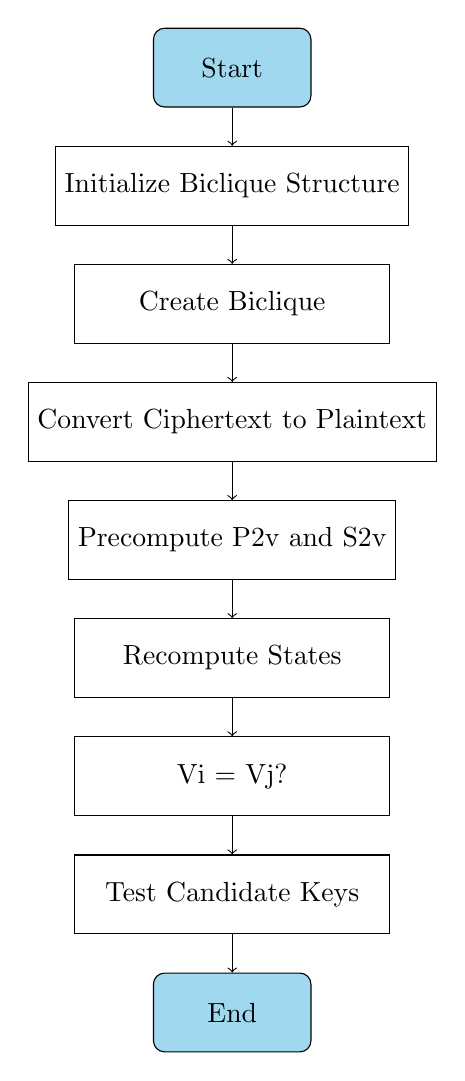
\begin{tikzpicture}[node distance=1.5cm]
    
        % Nodes
        \node (start) [draw, fill=lightblue, rounded corners, text centered, minimum height=1cm, minimum width=2cm] {Start};
        \node (init) [below of=start, draw, text centered, minimum height=1cm, minimum width=4cm] {Initialize Biclique Structure};
        \node (biclique) [below of=init, draw, text centered, minimum height=1cm, minimum width=4cm] {Create Biclique};
        \node (convert) [below of=biclique, draw, text centered, minimum height=1cm, minimum width=4cm] {Convert Ciphertext to Plaintext};
        \node (precompute) [below of=convert, draw, text centered, minimum height=1cm, minimum width=4cm] {Precompute P2v and S2v};
        \node (recompute) [below of=precompute, draw, text centered, minimum height=1cm, minimum width=4cm] {Recompute States};
        \node (compare) [below of=recompute, draw, fill=white, text centered, minimum height=1cm, minimum width=4cm] {Vi = Vj?};
        \node (testkeys) [below of=compare, draw, text centered, minimum height=1cm, minimum width=4cm] {Test Candidate Keys};
        \node (end) [below of=testkeys, draw, fill=lightblue, rounded corners, text centered, minimum height=1cm, minimum width=2cm] {End};
        
        % Arrows
        \foreach \i/\j in {start/init, init/biclique, biclique/convert, convert/precompute, precompute/recompute, recompute/compare, compare/testkeys, testkeys/end} {
            \draw[->] (\i) -- (\j);
        }
        
    \end{tikzpicture}
\end{center}

\subsection{Key Components}

\subsubsection{Biclique Structure}
The biclique structure is represented by the \texttt{BICL} struct, which maintains:
\begin{itemize}
    \item Current state (\texttt{S[SSize]})
    \item Ciphertext (\texttt{C[CSize]})
    \item Plaintext (\texttt{P[PSize]})
    \item Biclique key (\texttt{BicliqueKey[KeySize]})
    \item Differential transitions (\texttt{Delta\_i[CSize]} and \texttt{Nabra\_j[SSize]})
    \item Forward and backward states (\texttt{f\_state} and \texttt{b\_state})
\end{itemize}

\subsubsection{Biclique Construction}
The biclique construction is implemented in the \texttt{createBiclique} function, which:
\begin{enumerate}
    \item Generates a base key using \texttt{KeyCreate}
    \item Constructs differential transitions using \texttt{Delta\_i\_Key} and \texttt{Nabra\_j\_Key}
    \item Maps intermediate states to ciphertexts using the constructed differentials
\end{enumerate}

\begin{center}
    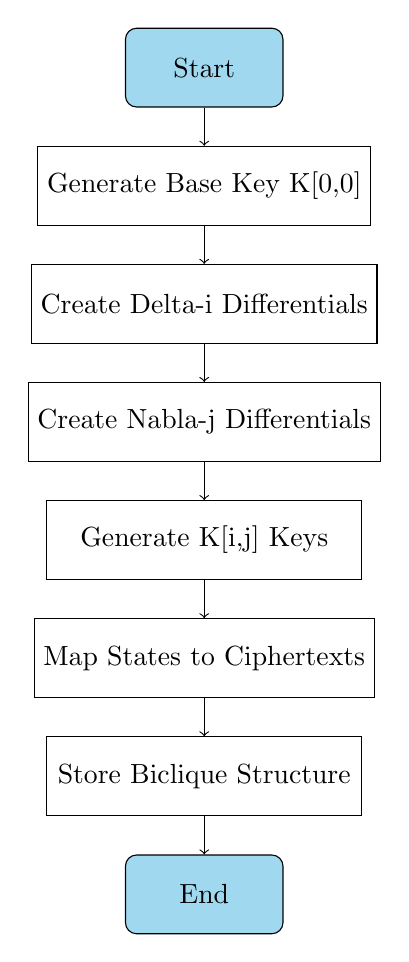
\begin{tikzpicture}[node distance=1.5cm]

        % Nodes
        \node (start) [draw, fill=lightblue, rounded corners, text centered, minimum height=1cm, minimum width=2cm] {Start};
        \node (generatebasekey) [below of=start, draw, text centered, minimum height=1cm, minimum width=4cm] {Generate Base Key K[0,0]};
        \node (createdelta) [below of=generatebasekey, draw, text centered, minimum height=1cm, minimum width=4cm] {Create Delta-i Differentials};
        \node (createnabla) [below of=createdelta, draw, text centered, minimum height=1cm, minimum width=4cm] {Create Nabla-j Differentials};
        \node (generatekeys) [below of=createnabla, draw, text centered, minimum height=1cm, minimum width=4cm] {Generate K[i,j] Keys};
        \node (mapstates) [below of=generatekeys, draw, text centered, minimum height=1cm, minimum width=4cm] {Map States to Ciphertexts};
        \node (storeresults) [below of=mapstates, draw, text centered, minimum height=1cm, minimum width=4cm] {Store Biclique Structure};
        \node (end) [below of=storeresults, draw, fill=lightblue, rounded corners, text centered, minimum height=1cm, minimum width=2cm] {End};
        
        % Arrows
        \foreach \i/\j in {start/generatebasekey, generatebasekey/createdelta, createdelta/createnabla, createnabla/generatekeys, generatekeys/mapstates, mapstates/storeresults, storeresults/end} {
            \draw[->] (\i) -- (\j);
        }
        
    \end{tikzpicture}
\end{center}


\subsection{Attack Implementation}
The attack follows these main steps:

\subsubsection{1. Precomputation Phase}
Two main precomputation functions are implemented:
\begin{itemize}
    \item \texttt{precompute\_P2v}: Computes forward transitions from plaintexts
    \item \texttt{precompute\_S2v}: Computes backward transitions from states
\end{itemize}

The precomputation reduces the computational complexity by storing intermediate results that can be reused during the attack.

\subsubsection{2. Recomputation Phase}
The \texttt{recompute} function implements the recomputation step, which:
\begin{itemize}
    \item Recomputes key schedules using \texttt{KeyRecompute}
    \item Updates forward states using \texttt{RecomputeF}
    \item Updates backward states using \texttt{RecomputeB}
\end{itemize}

\subsubsection{3. Key Testing}
The \texttt{testCandidateKeys} function verifies potential key candidates by:
\begin{enumerate}
    \item Decrypting ciphertexts using candidate keys
    \item Comparing results with known plaintexts
    \item Identifying matching keys as potential solutions
\end{enumerate}

\includesvg{figures/keyflow.svg}
\begin{verbatim}
%% Output sample: Vi=Vj
---
Possible key here: K[81][36]
9a,de,ca,2,fa,37,9b,bc,2b,d2,65,7b,5f,7e,bb,39
Vi is : b8	Vj is : b8
\end{verbatim}

\begin{verbatim}
%% Output Sample: P=P'?
Known plaintext for K[81][36]: 3f 25 3f 1a af 90 28 8c 79 12 4 eb d4 e0 b 27 
Testing candidate key K[81][36]: 9a de ca 2 fa 37 9b bc 2b d2 65 7b 5f 7e bb 39 
Decrypted plaintext: ee cc e2 27 3c b1 60 d5 15 7e 55 56 8e 22 59 43
\end{verbatim}

\subsection{Performance Considerations}
Our implementation includes several optimizations:
\begin{itemize}
    \item Efficient key schedule computation
    \item Minimized state transitions
    \item Optimized memory usage for state storage
\end{itemize}

\subsection{Limitations}
The current implementation has several limitations:
\begin{itemize}
    \item Focuses only on rounds 8-10 of AES
    \item Uses a fixed dimension ($d = 8$) for the biclique
    \item Requires significant memory for state storage
    \item Does not implement all optimizations from the theoretical attack
\end{itemize}

\subsection{Testing and Validation}
The implementation includes a validation function \texttt{validateAESImplementation} that:
\begin{itemize}
    \item Verifies correct AES operation
    \item Tests biclique construction
    \item Validates key recovery functionality
\end{itemize}

Test results demonstrate successful attack for key recovery for the implemented rounds, though with higher computational complexity than theoretical bounds due to implementation simplifications. Although there has not been any successful recovery of key achieved by this code, several factors impacts this including computation limitations and possible mistakes during implementation.


\bibliographystyle{plain} % You can choose other styles like IEEEtran, alpha, etc.
\bibliography{references}
\end{document}
